\documentclass{mcmthesis}
\mcmsetup{CTeX = true,   % 使用 CTeX 套装时,设置为 true
        tcn = 0000, problem = B,
        sheet = true, titleinsheet = true, keywordsinsheet = true,
        titlepage = true, abstract = true}
\usepackage{palatino}
\usepackage{subfigure}
\usepackage[UTF8, nocap]{ctex}
\usepackage{algorithm}
\usepackage{algorithmicx}
\usepackage{algpseudocode}
\usepackage{lipsum}
\title{Modeling merge after toll}
%\author{\small Tom}
\date{\today}
\begin{document}
\begin{abstract}
\lipsum[1]
\begin{keywords}
keyword1; keyword2
\end{keywords}
\end{abstract}
\maketitle
\tableofcontents
\newpage
\section{Introduction}
%如何将交通流量进行有效的合并是交通史上历来备受关注的问题,
高速公路的收费站会通过过卡收费的方式收取驾驶员的高速费,过卡收费时,由于收费窗口的数量通常要比车道数量多,因此当汽车交费后从收费站驶出时,车流必须从较宽的呈扇形收费站广场快速并入较少的常规的机动车车道,收费广场的建立就是为了解决在这个过程中产生的拥堵现象。优化收费广场的建立方案,使得在更小的占地面积内达到最高的交通效率。


为了增强车辆通行能力,增大吞吐量,减小交通事故发生的可能性,简单的解决方式就是增加收费广场长度,以减小并线压力,增加长度同样也增大了收费广场的面积,但收费广场面积越大,建设成本也会随之升高,因而需要寻找在车辆通行能力最佳的条件下,使得收费站形状最优、大小最小的收费站区域设计方案。除此之外,车道合并的模式对收费站的形状大小起着决定作用,因而对合并车道方案进行详细说明,评价方案包括下列指标。

\begin{itemize}
	\item 不同合并方式下的出流量。
	\item  不同合并方式所占用的面积。
\end{itemize}

我们研究了在不同形状、大小、合并方式的情况下对收费站拥堵情况的影响,提出了基于离散化车流密度的元胞自动机模型。

对于电子收费窗口,与不找零收费窗口,由于其通过速度快,可能反而会造成合并区域的拥堵现象\cite{spiliopoulou2009toll}。
到目前为止,全世界绝大部分地区的收费方式存在人工收费窗口与电子收费窗口比例不协调的现象,这使得过多电子收费窗口闲置而人工收费窗口拥堵。通过收费窗口后,几乎所有收费广场都是采取扇形区域来实施汽车的合流,因此当遇到高峰时,收费广场拥堵现象仍然普遍存在。

自动驾驶是一项新兴技术,随着自动驾驶汽车数量逐渐增加,由于自动驾驶技术的特性,道路容量将会下降


%%%%%%%%%%%%%%%%%%%%%%%%%%%%%%%%%%%%%%%%%%%

\subsection{Other Assumptions}
为了简化模型,我们做出了如下假设
\begin{itemize}
\item 假设从收费站驶出的车流量分布为泊松分布。
\item 假设高速公路的出入分别是分离的。
\item 
\item
\end{itemize}

\lipsum[7]

\section{Analysis of the Problem}
%设有如下高速公路收费站汇合区域,收费站有B个收费窗口,汇合到有L条车道的高速公路。
收费站区域一般都为扇形区域,如图所示,收费站B条出口,并入L条常规路线,其中B大于L。
Toll merge area show as \ref{fig:merge_area},\cite{woo1991toll}
\begin{figure}[!h]
	\centering
	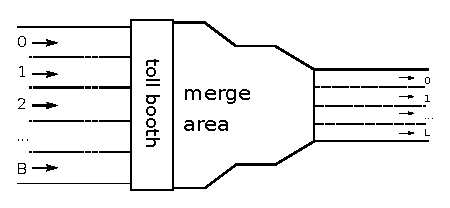
\includegraphics[width=0.5\textwidth]{merge_area.eps}
	\caption{merge area}
	\label{fig:merge_area}
\end{figure}
我们假设所有通过收费窗口的车流分布程泊松分布,即越靠近中间车道的收费窗口通过的车流量越大。
从收费站通过在扇形区域的合并模式,由于收费站广场的长度不同,分为两种合并方式。
单次并道与多次并道,由合并位置的不同分为单侧并道与双侧并道,
如Figure \ref{fig:merge_ways}所示。
%我们考虑了三种合并方式,直接合并,单侧多次合并,双侧多次合并,示意图如下:
We had considered 3 way to merge, 1) direct merge, 2) single side multiple merge, 3) double side multiple merge.
\begin{figure}[!htbp]
	\centering
	\subfigure[single merging]{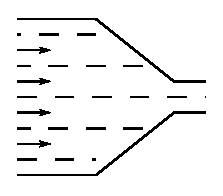
\includegraphics[width=0.3\textwidth]{ws_merge.eps}}
	\subfigure[one-side mutiple mering]{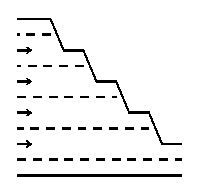
\includegraphics[width=0.3\textwidth]{ss_merge.eps}}
	\subfigure[double-side multiple merging]{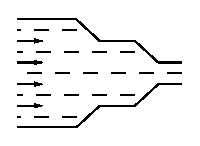
\includegraphics[width=0.3\textwidth]{ds_merge.eps}}
	\caption{merging ways}
	\label{fig:merge_ways}
\end{figure}
衡量收费窗口通行能力的主要因素就是考虑车辆通过收费广场的最大通行容量,即最大不发生拥堵的车流量,将合并区域离散化,建立元胞自动机模型。
\subsection{建立模型}
车辆通过收费窗口之后,车流量对于收费窗口的分布服从泊松分布.为定量模拟收费广场合并时广场形状和面积对车流量的影响,将收费广场网格化,分割成为有限个、状态连续的单元格,每一小格可近似看作一个单元(unit),每个单元的取值为该单元的车流量(“元胞”的车流量定义为单位时间内在该元胞上通过的机动车数量)。散布在规则格网中的每一单元都遵循同样的运动规则,依据确定的局部规则作同步更新。大量元胞通过简单的相互作用而构成动态系统的演化。
由左侧第一列产生进入流量Q,所有流量的传播方向如Figure \ref{fig:road_dis}所示。
%将路口分布看为离散化如下图
%箭头的方向代表车流量可能的方向
\begin{figure}[h]
\small
\centering
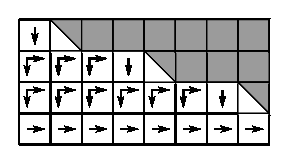
\includegraphics[width=0.5\textwidth]{road_dis.eps}
\caption{road discrete} 
\label{fig:road_dis}
\end{figure}
所有单元按照传播方向与周围格子的状态决定传播流量,传播流量的大小由传播函数控制,如Equation \ref{eq:s_func}所示。
\begin{equation}
f=\frac{1}{1+e^{3q-7}}
\label{eq:s_func}
\end{equation}
图像如Figure \ref{fig:s_func}所示。每个单元格达到4的车流量视为饱和。
\begin{figure}[!htbp]
	\small
	\centering
	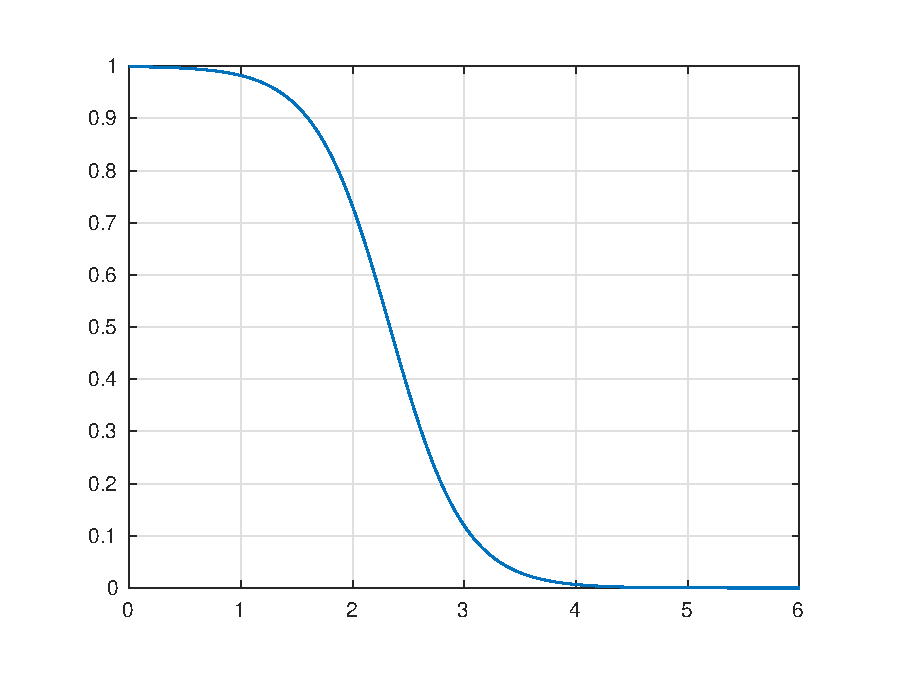
\includegraphics[width=0.5\textwidth]{sfunc.eps}
	\caption{s function} 
	\label{fig:s_func}
\end{figure}
如果某单元格只有一个传播方向,那么此单元格只需简单通过传播函数决定传播流量的多少到下一个单元格;若某单元格具有不同的选择,即有两个传播方向,单元格首先会根据传播方向上的流量的不同而决定一个主要的传播方向,比如:如果某单元格下方流量较少而前方流量较多,则传播流量的主要部分会集中在下方,伪代码如Algorithm \ref{alg:flow_ctl}所示:
\begin{algorithm}
	\begin{algorithmic}
	\caption{Flow Control}
	\label{alg:flow_ctl}
        \Require $\text{本格流量q,前方一格流量ql,下方一格流量qd}$
		\Ensure $\text{流量控制结果}$
		\Function {FlowCtl}{$q, qd, ql$}
				\If {$qd < ql$}
					\State $q,qd \gets \Call{downward}{q,qd}$
					\State $q,ql \gets \Call{forward}{q,ql}$
				\Else
					\State $q,ql \gets \Call{forward}{q,ql}$
					\State $q,qd \gets \Call{downward}{q,qd}$
			\EndIf
			\State \Return{$q,qd,ql$}
		\EndFunction
\end{algorithmic}
\end{algorithm}

当道路流量上升时,发生事故的概率也会增大,
ETC may lead\cite{spiliopoulou2009toll}

\section{The Model Results}
\subsection{并道方式选择}
结合所建立的模型,为求解合并区域的最优形状,定量分析当B=10,L=2时进行仿真,结果如下。
\subsubsection{单次并道}
单次并道是指从高速收费亭的B个收费口出来到L个车道的高速公路的过程中,只需要一次车道合并。在此种情况下,在合并过程中,多个车道同时合并,容易发生交通事故,且多车同时并道容易造成道路拥挤。通过以上建立的模型利用matlab仿真实现,如Figure \ref{fig:direct_out}所示。
最终出流量为$71.4$。
\begin{figure}[!htbp]
	\small
	\centering
	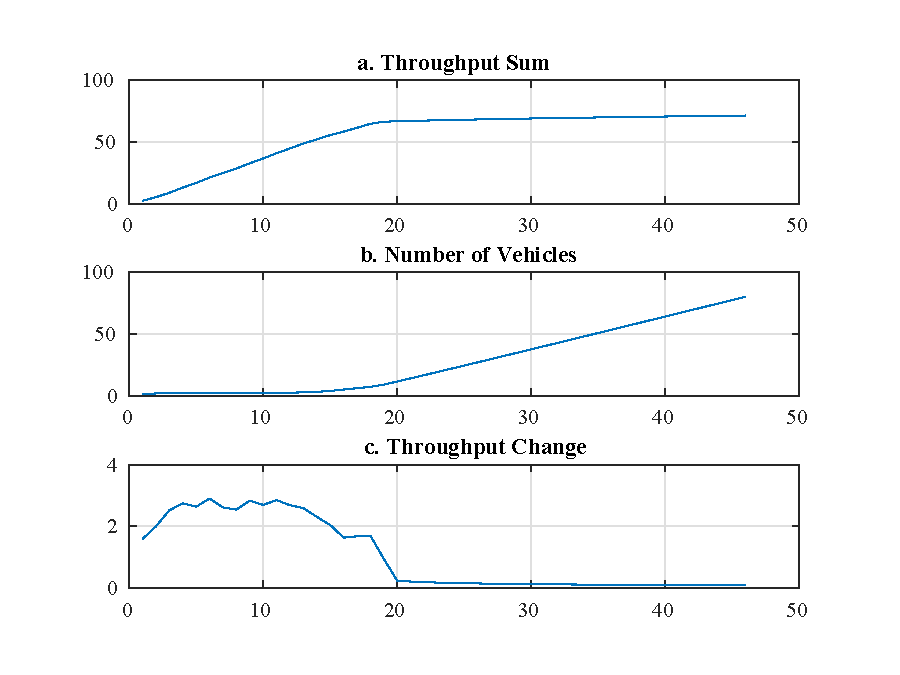
\includegraphics[width=0.8\textwidth]{sssout.eps}
	\caption{direct out} 
	\label{fig:direct_out}
\end{figure}
\subsubsection{多次并道}
多次并道是指从高速收费亭的B个收费口出来需要多次车道合并才能到达L个车道的高速公路的并道模式。在此种情况下,道路合并次数可以根据高速公路的车道数而定,且在并道过程中,机动车驾驶人可选择道路中车辆数少且更加便捷的路线并道,即更加便捷、选择更多的减少交通事故的发生。在此情况下,可对单侧并道、双侧并道的情形分别研究,通过matlab程序实现,结果Figure \ref{fig:multiple_out}所示。
最终出流量为$93.1$。
\begin{figure}[!htbp]
	\small
	\centering
	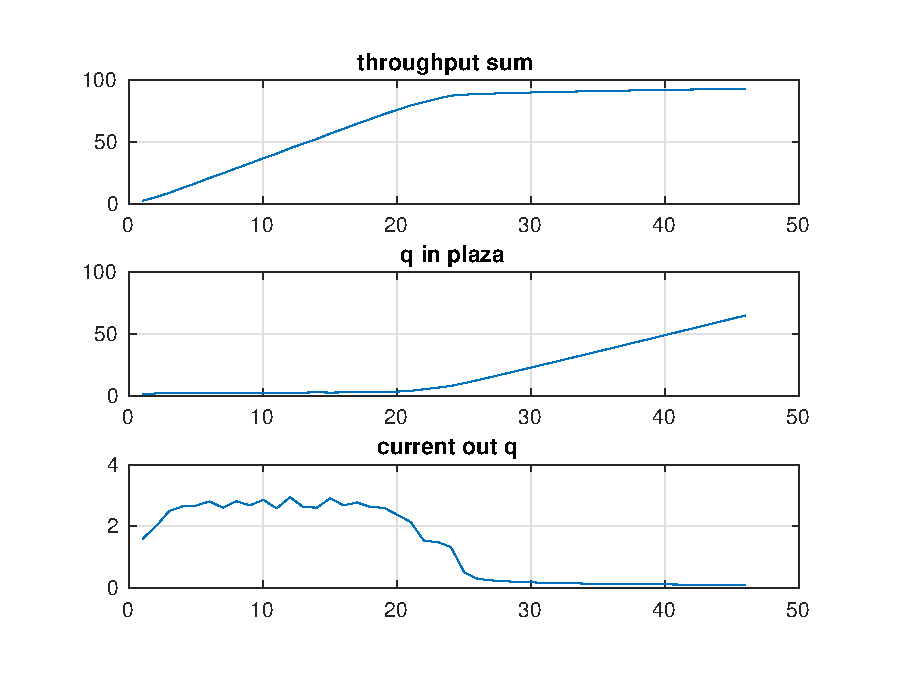
\includegraphics[width=0.8\textwidth]{dssout.eps}
	\caption{multiple out} 
	\label{fig:multiple_out}
\end{figure}

以上结果显示,适当增加合并区域的长度,会有效改善道路的通行能力,
\subsection{车流量大小的影响}
当车流量较小时,道路通行能力维持在最高水平。
\lipsum[9]
\begin{figure}[!htbp]
	\small
	\centering
	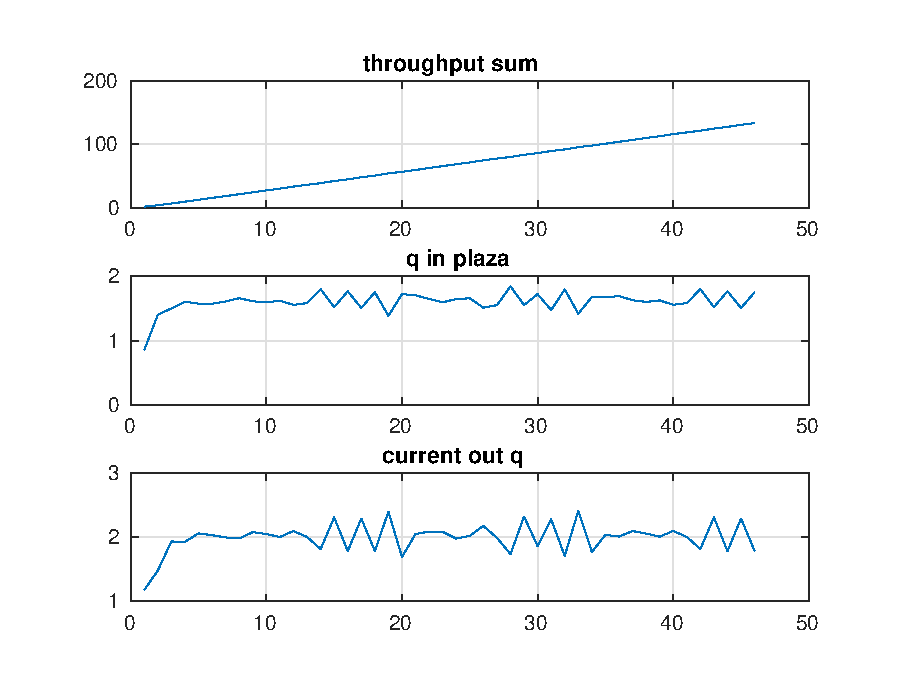
\includegraphics[width=0.8\textwidth]{low_q.eps}
	\caption{low q} 
	\label{fig:q_low}
\end{figure}

当车流量较高时,道路通行能力很快饱和。
\begin{figure}[!htbp]
	\small
	\centering
	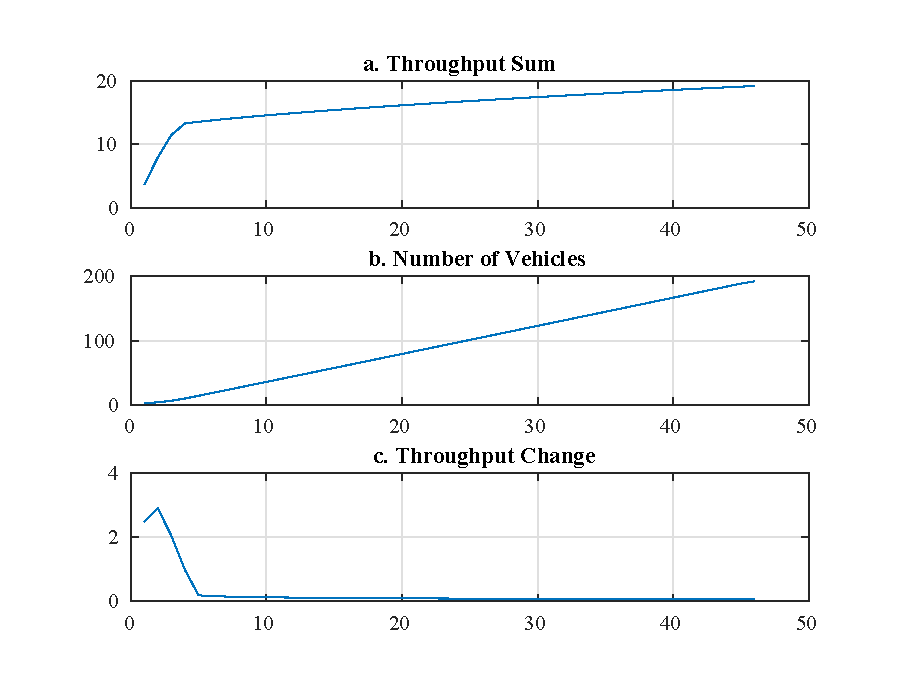
\includegraphics[width=0.8\textwidth]{high_q.eps}
	\caption{high q} 
	\label{fig:q_high}
\end{figure}
\subsection{事故预防}
由仿真得到交通密度如Figure \ref{fig:q_map}所示。
\begin{figure}[!htbp]
	\small
	\centering
	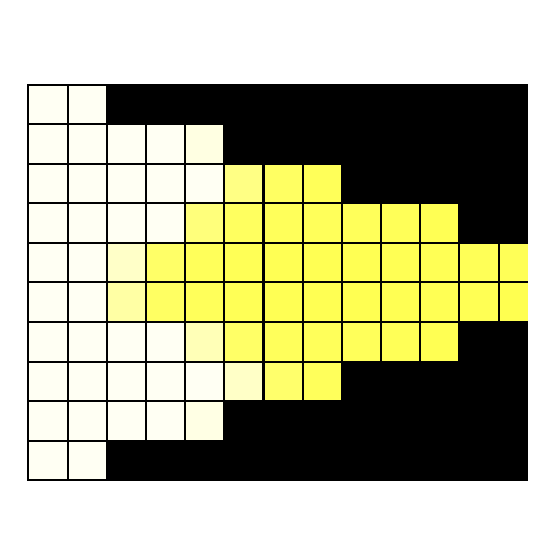
\includegraphics[width=0.8\textwidth]{q_map.eps}
	\caption{q map} 
	\label{fig:q_map}
\end{figure}
根据流量判断哪条道路上发生事故的概率更高,提前做好预防。

\subsection{自动驾驶车辆的影响}
加入自动驾驶车辆后,会使道路饱和密度降低,

\subsection{电子支付通道的影响}
增加电子支付通道,会提高该道路的流量。下图是开通之后
\begin{figure}[!htbp]
	\small
	\centering
	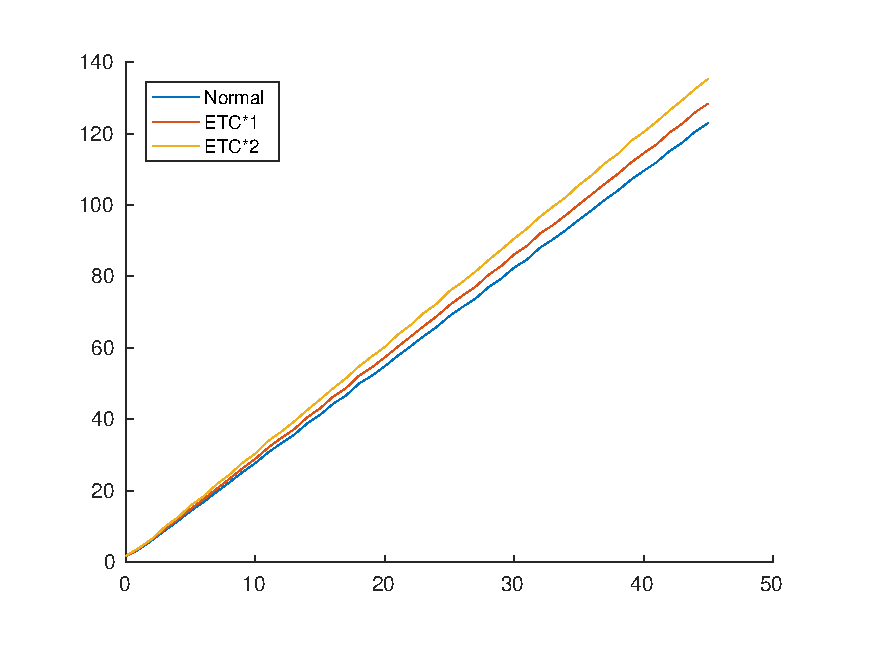
\includegraphics[width=0.8\textwidth]{etc.eps}
	\caption{etc} 
	\label{fig:etc}
\end{figure}
\section{Conclusions}
\lipsum[6]

\section{Evaluate of the Mode}

\section{Strengths and weaknesses}
\lipsum[12]

\subsection{Strengths}
\begin{itemize}
\item \textbf{Applies widely}\\
This  system can be used for many types of airplanes, and it also
solves the interference during  the procedure of the boarding
airplane,as described above we can get to the  optimization
boarding time.We also know that all the service is automate.
\item \textbf{Improve the quality of the airport service}\\
Balancing the cost of the cost and the benefit, it will bring in
more convenient  for airport and passengers.It also saves many
human resources for the airline. \item \textbf{}
\end{itemize}

\newpage
\bibliography{mybib}
\bibliographystyle{plain}
\newpage

%\begin{thebibliography}{99}
%\bibitem{1} A
%\end{thebibliography}

\begin{appendices}

\section{First appendix}

\lipsum[13]

Here are simulation programmes we used in our model as follow.\\

\textbf{\textcolor[rgb]{0.98,0.00,0.00}{Input matlab source:}}
\lstinputlisting[language=Matlab]{./code/mcmthesis-matlab1.m}

\section{Second appendix}

some more text \textcolor[rgb]{0.98,0.00,0.00}{\textbf{Input C++ source:}}
\lstinputlisting[language=C++]{./code/mcmthesis-sudoku.cpp}

\end{appendices}
\end{document}
